% !TeX encoding = UTF-8
\chapter{Client}
\thispagestyle{fancy}
\label{client}



\section{Grafische Benutzeroberfläche (GUI)}

Die Gestaltung dieser GUI bezweckt eine leicht verständliche intuitiv bedienbare Oberfläche mit zielführender Benutzerführung und Hilfestellungen.
Die GUI ist für Geräte mit Android als Betriebssystem entwickelt, aber theoretisch nach dem kompilieren mit eventuell erforderlichen kleinen Anpassung auch auf andere Plattformen/Geräten ähnlich abgebildet und verwendbar. Erfolgreich getestet ist die App allerdings derzeit nur für Android (4.3 + 4.4) und Windows.

\begin{figure}[ht!]
	\centering
	\begin{minipage}{0.31\linewidth}
		\centering
		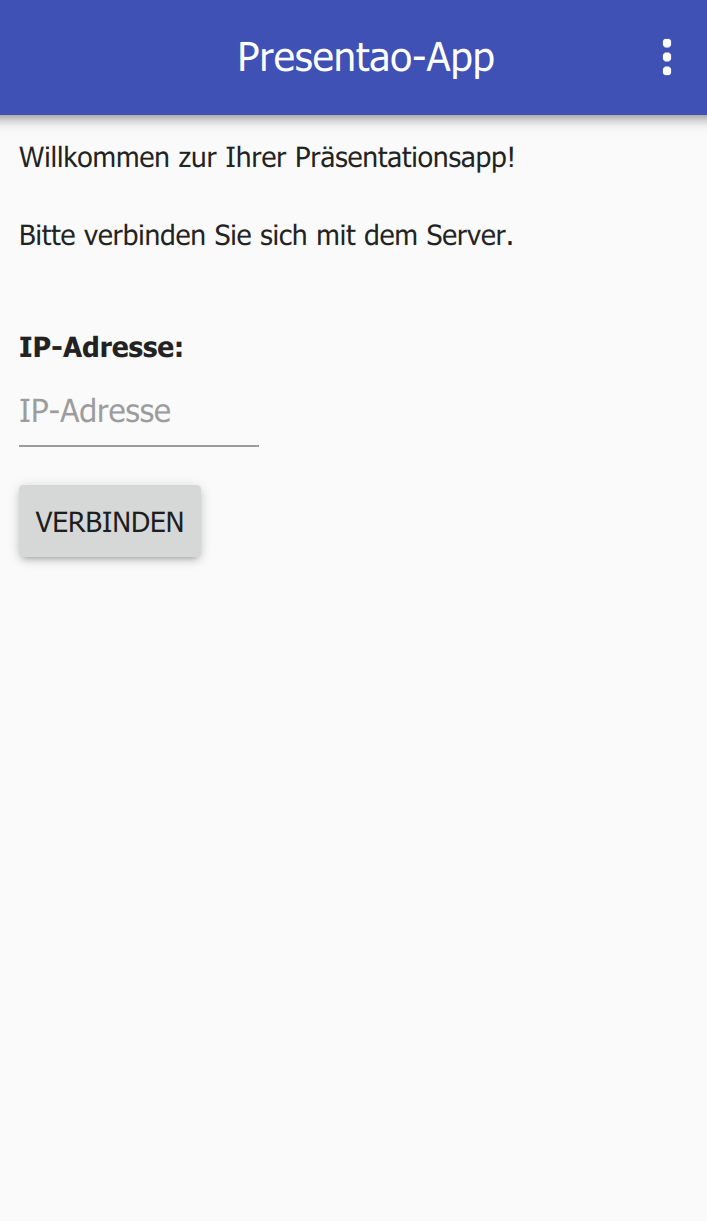
\includegraphics[scale=0.5]{GUI/Bilder/1_Startbildschirm.PNG}
	\end{minipage}
	%\hfill
	\begin{minipage}{0.31\linewidth}
		\centering
		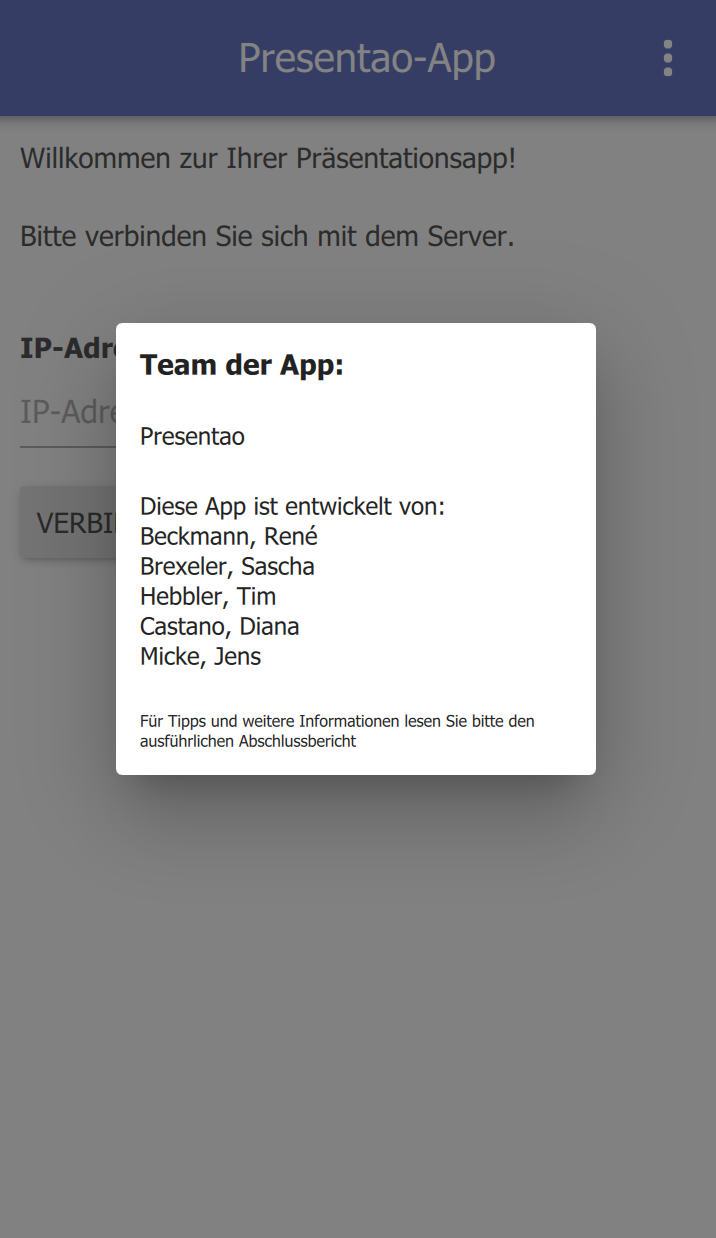
\includegraphics[scale=0.5]{GUI/Bilder/1_0_1_Startbildschirm_PopUP_Team.PNG}
	\end{minipage}
	\begin{minipage}{0.31\linewidth}
		\centering
		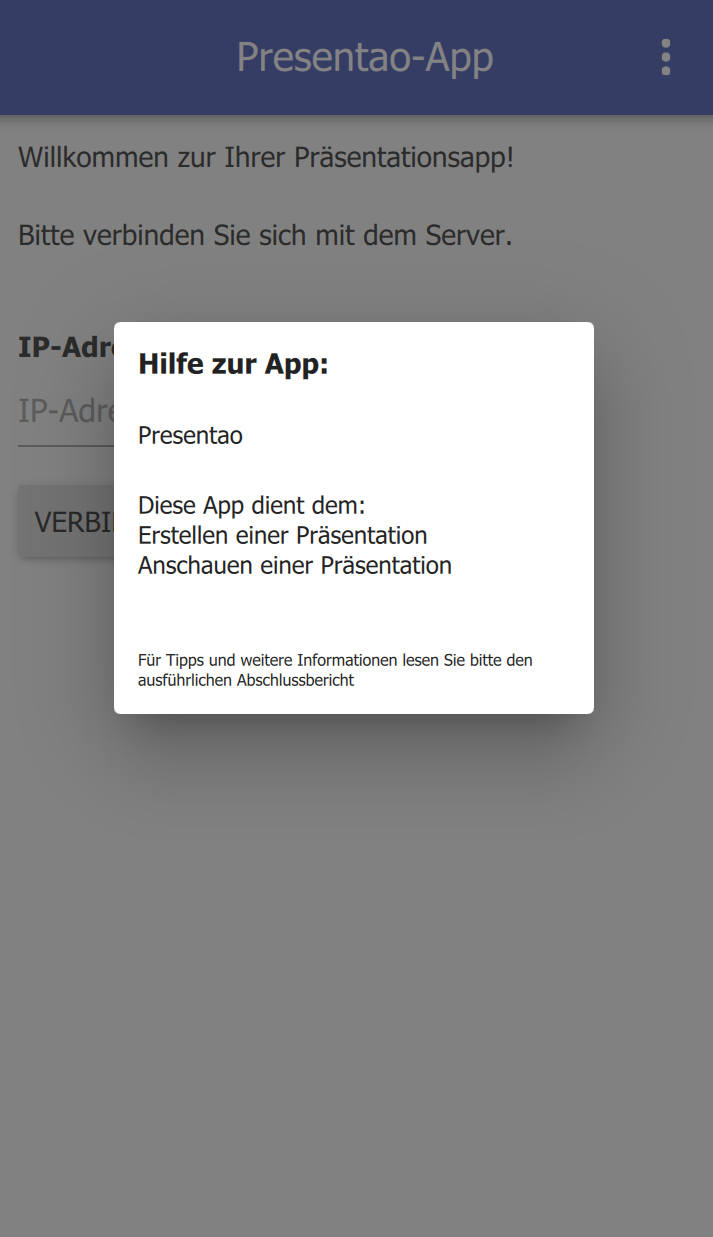
\includegraphics[scale=0.5]{GUI/Bilder/1_0_1_Startbildschirm_PopUP_Hilfe.PNG}
	\end{minipage}
	\caption{v.l.n.r.: Startbildschirm, Über die App, Hilfemenü{\tiny}}
	\label{client:Appstart}
\end{figure}

\newpage

\paragraph{Start der App}$\;$\\
Von dem Startbildschirm aus besteht die Möglichkeit ein Menü (siehe \autoref{client:OptionsMenue}) durch klicken auf den aus drei Punkten bestehenden Menü-Button (siehe \autoref{client:Appstart}) aufzurufen.
\\In diesem lassen sich zwei Pop-Ups zur Hilfe und zum Team aufrufen (siehe \autoref{client:Appstart}).
\begin{figure}[ht!]
	\centering
	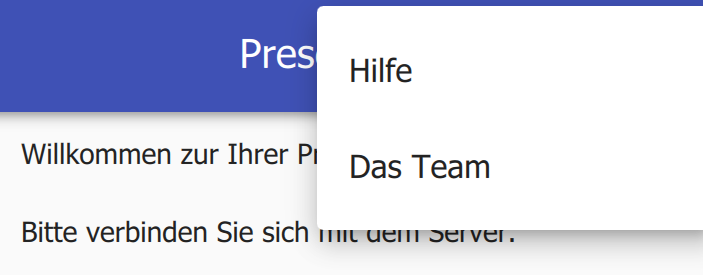
\includegraphics[scale=0.5]{GUI/Bilder/Info_Menu.PNG}
	\caption{Menü{\tiny}}
	\label{client:OptionsMenue}
\end{figure}
\paragraph{Verbindungsaufbau}$\;$\\
Des Weiteren kann der Benutzer nach Eingabe einer der gültigen IP-Adresse eine Verbindung zum Server als Zuhörer aufbauen. Die Eingabe der IP-Adresse erfolgt, wie in der üblichen Notation, mit Punkttrennung und eine Portangabe ist nicht nötig, da diese in Client und Server fest einprogrammiert ist.

\begin{figure}[ht!]
	\centering
	\begin{minipage}{0.31\linewidth}
		\centering
		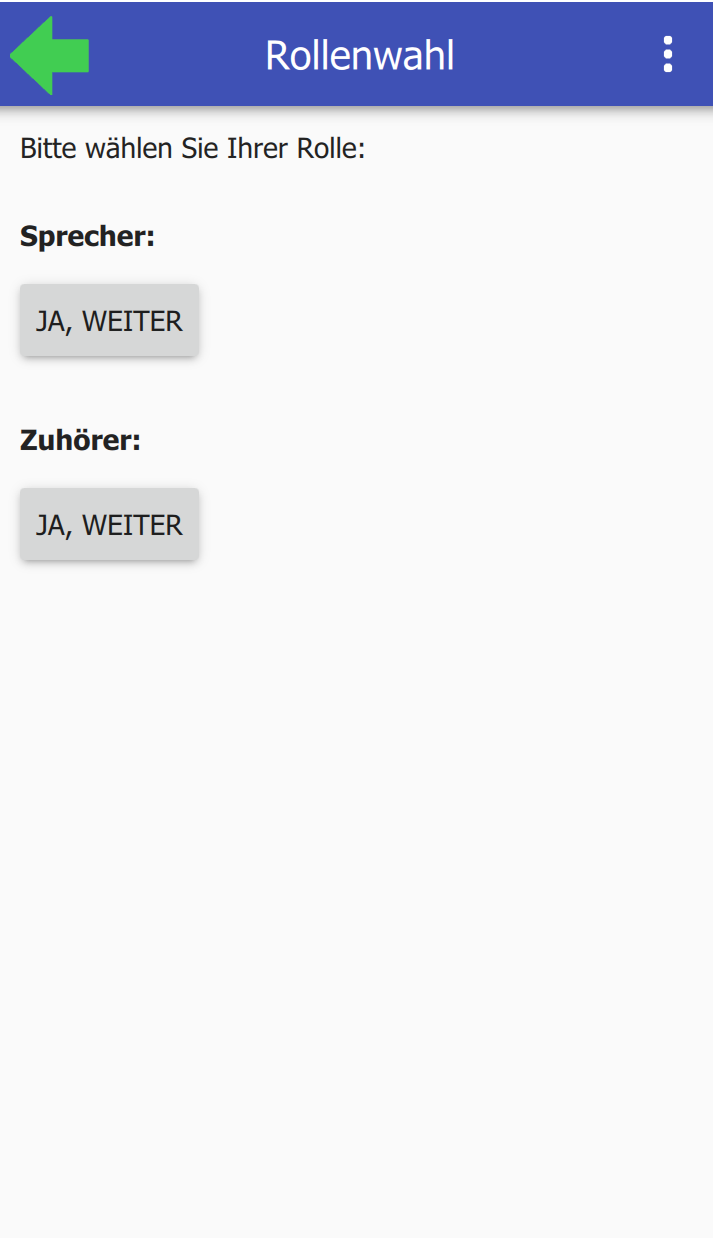
\includegraphics[scale=0.5]{GUI/Bilder/2_Rollenwahl.PNG}
	\end{minipage}
	%\hfill
	\begin{minipage}{0.31\linewidth}
		\centering
		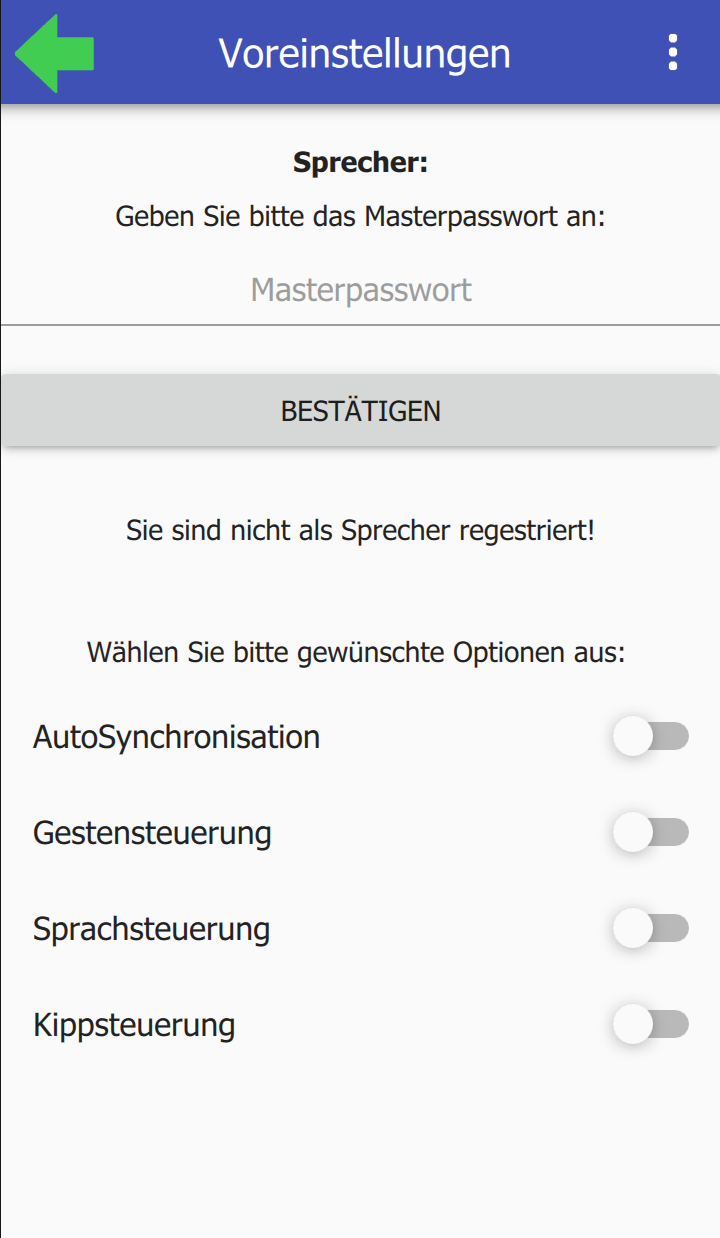
\includegraphics[scale=0.5]{GUI/Bilder/3_S_1_Voreinstellung.PNG}
	\end{minipage}
	\begin{minipage}{0.31\linewidth}
		\centering
		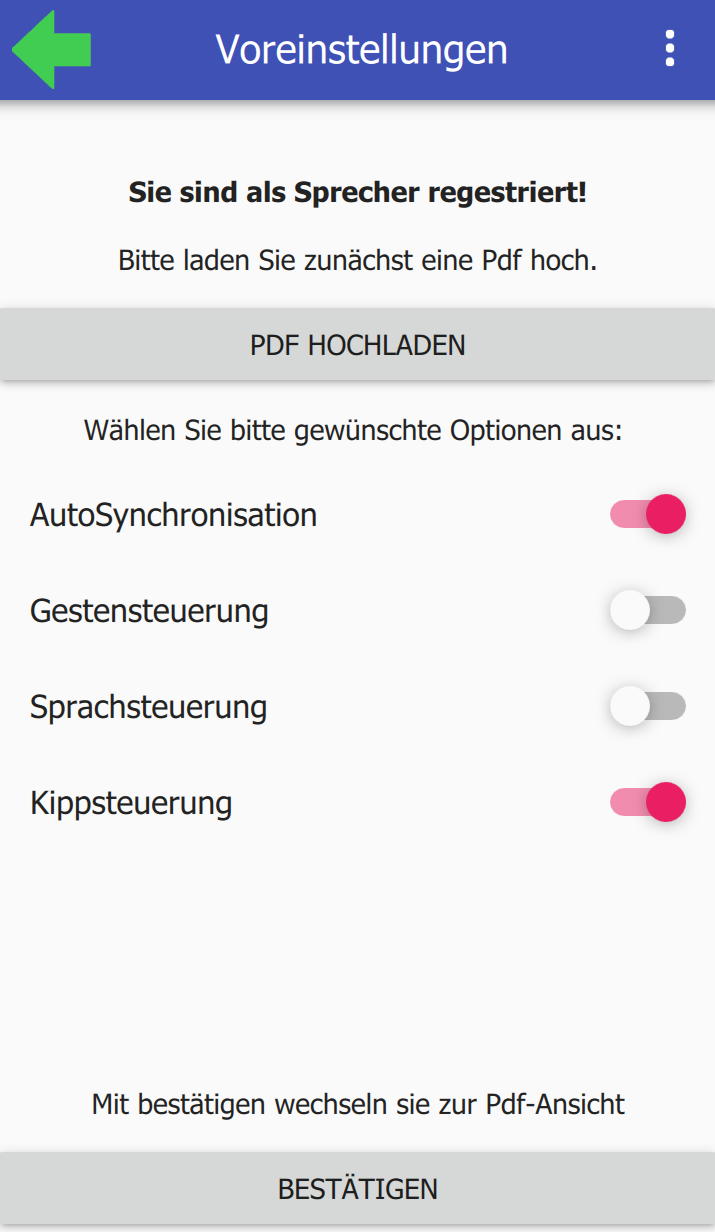
\includegraphics[scale=0.5]{GUI/Bilder/3_S_5_Voreinstellung.PNG}
	\end{minipage}
	\caption{v.l.n.r.: Rollenwahl, Voreinstellungen des Sprecher vor und nach Registrierung{\tiny}}
	\label{client:Rollenauswahl+S_Voreinstellungen}
\end{figure}

\newpage

\paragraph{Auswählen der eigenen Rolle}$\;$\\
Nach erfolgreichen Verbindungsaufbau wechselt die Ansicht in zur Rollenauswahl. Ein Label zeigt diese Position mittig der oberen Leiste (Toolbar) an (siehe \autoref{client:Rollenauswahl+S_Voreinstellungen}).
In dieser Toolbar befindet sich nun zusätzlich ein grüner Pfeil nach links, um zur vorherigen Ansicht zu wechseln.
\\Die Rollenwahl ist wiederholbar und somit korrigierbar, aber unumgänglich implementiert, da weitere Einstellung und Möglichkeiten auf dieser Entscheidung aufbauen.
\paragraph{Voreinstellungen als Sprecher}$\;$\\
Der Sprecher muss sich zunächst als solcher bei dem Server registrieren. Dazu ist eine Passwortabfrage eingerichtet. Das sog. Masterpasswort ist "mpw12345". Wenn die Eingabe fehlerhaft erfolgte, erscheint zusätzlich unter dem Textfeld zur Passworteingabe (siehe \autoref{client:Rollenauswahl+S_Voreinstellungen}) in Dickschrift der Hinweis: "Bitte überprüfen Sie Ihre Passworteingabe". Sobald die Eingabe richtig und bestätigt ist, kann der Benutzer eine Pdf-hochgeladen. Dazu muss der Nutzer eine Pdf-Datei über den File-Dialog (siehe \autoref{client:FileDialog}) suchen und auswählen. Eine Erfolgreiche Auswahl sendet die Datei an den Server, der diese direkt an über den Projektor auf Seite 0 ausgibt. Bevor der Sprecher mit Bestätigen zur Pdf-Ansicht wechselt, sieht dieser noch eine Liste (ListView) mit einige Optionen aus denen er gewünschte über Schiebeschalter (SwitchDelegates) auswählen kann. Mit dem grünen Pfeil wechselt die Ansicht diesmal zurück zur Rollenwahl.

\begin{figure}[ht!]
	\centering
	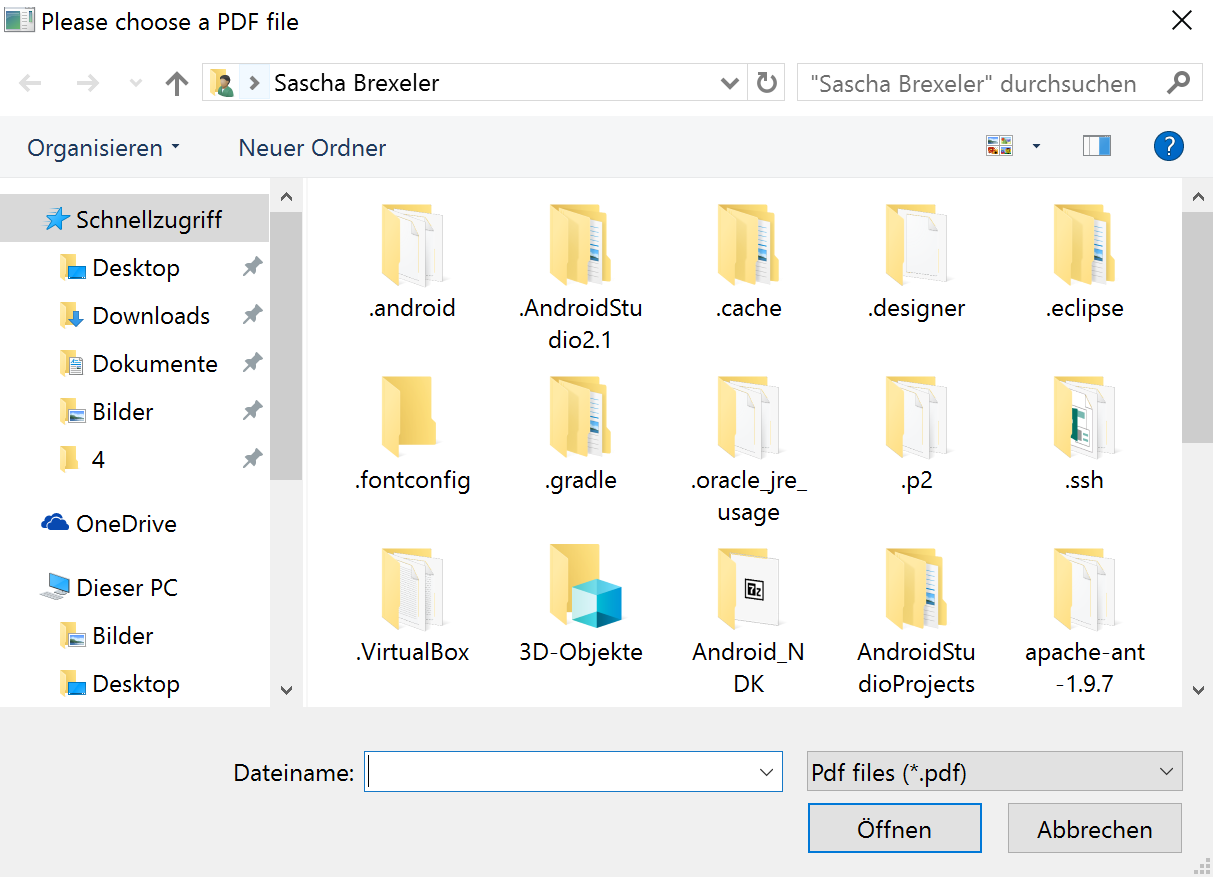
\includegraphics[scale=0.7]{GUI/Bilder/3_S_4_Voreinstellung.PNG}
	\caption{File-Dialog{\tiny}}
	\label{client:FileDialog}
\end{figure}

\begin{figure}[ht!]
	\centering
	\begin{minipage}{0.31\linewidth}
		\centering
		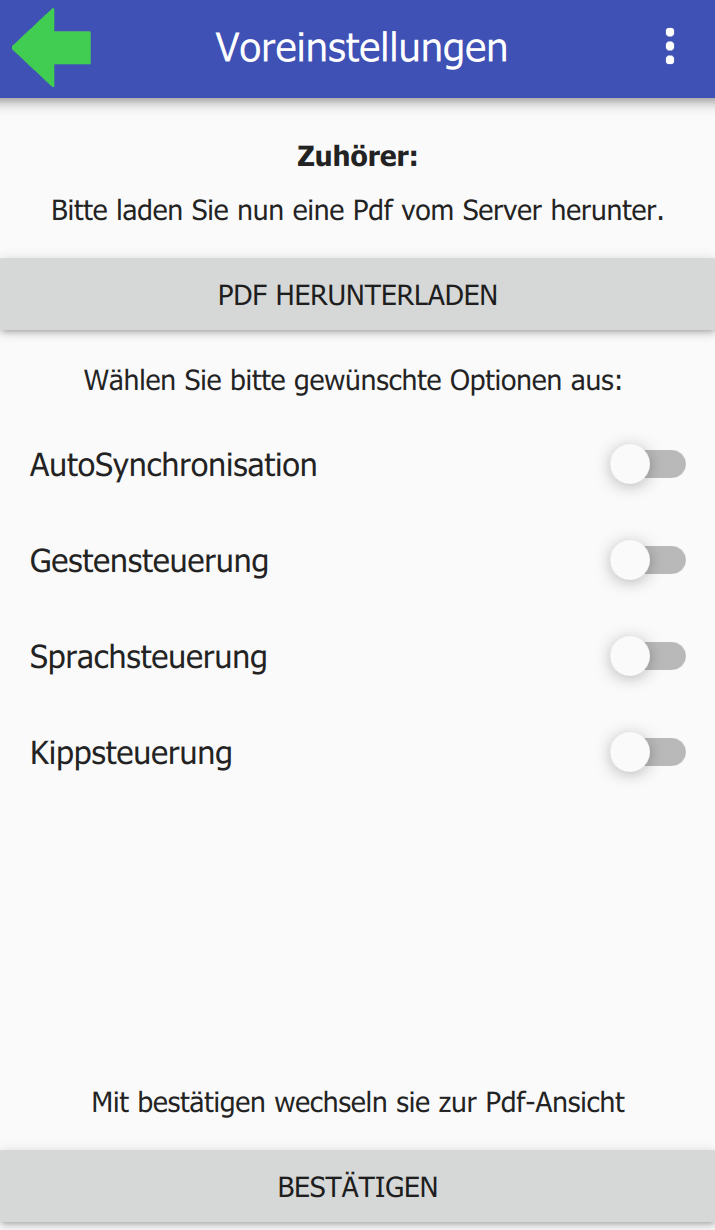
\includegraphics[scale=0.5]{GUI/Bilder/7_H_Voreinstellungen.PNG}
	\end{minipage}
	%\hfill
	\begin{minipage}{0.31\linewidth}
		\centering
		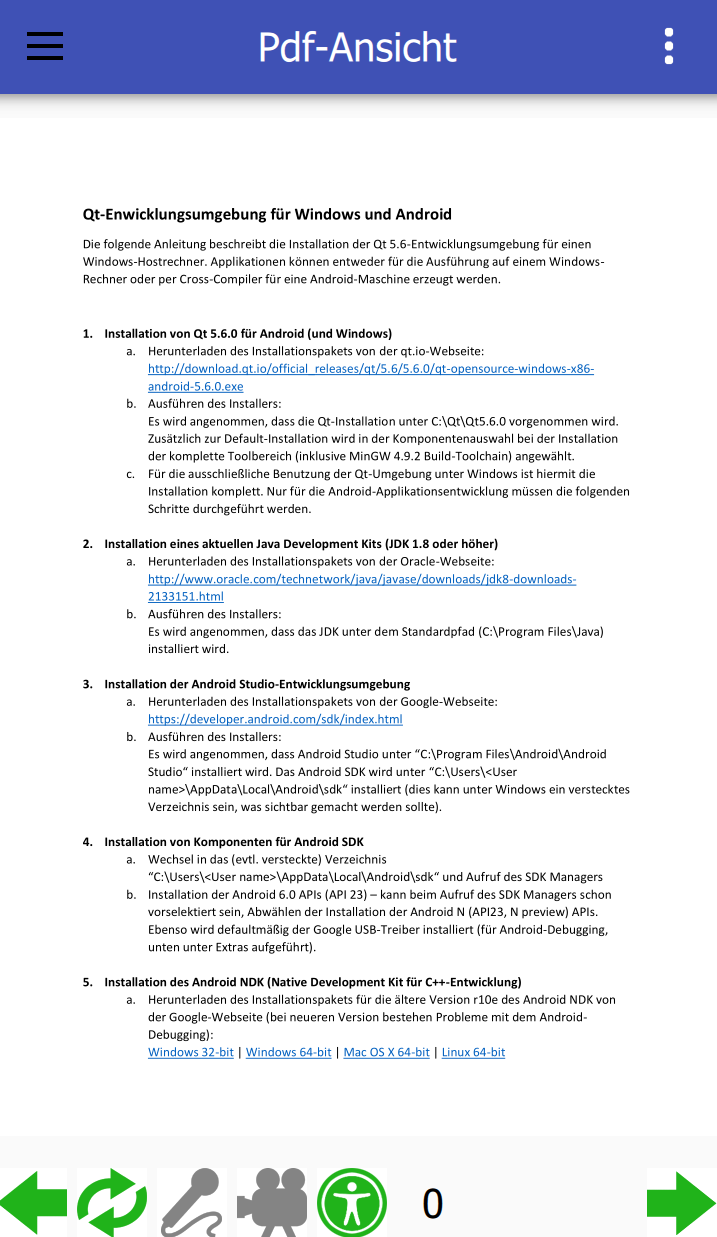
\includegraphics[scale=0.5]{GUI/Bilder/4_S_PDF-Ansicht.PNG}
	\end{minipage}
	\begin{minipage}{0.31\linewidth}
		\centering
		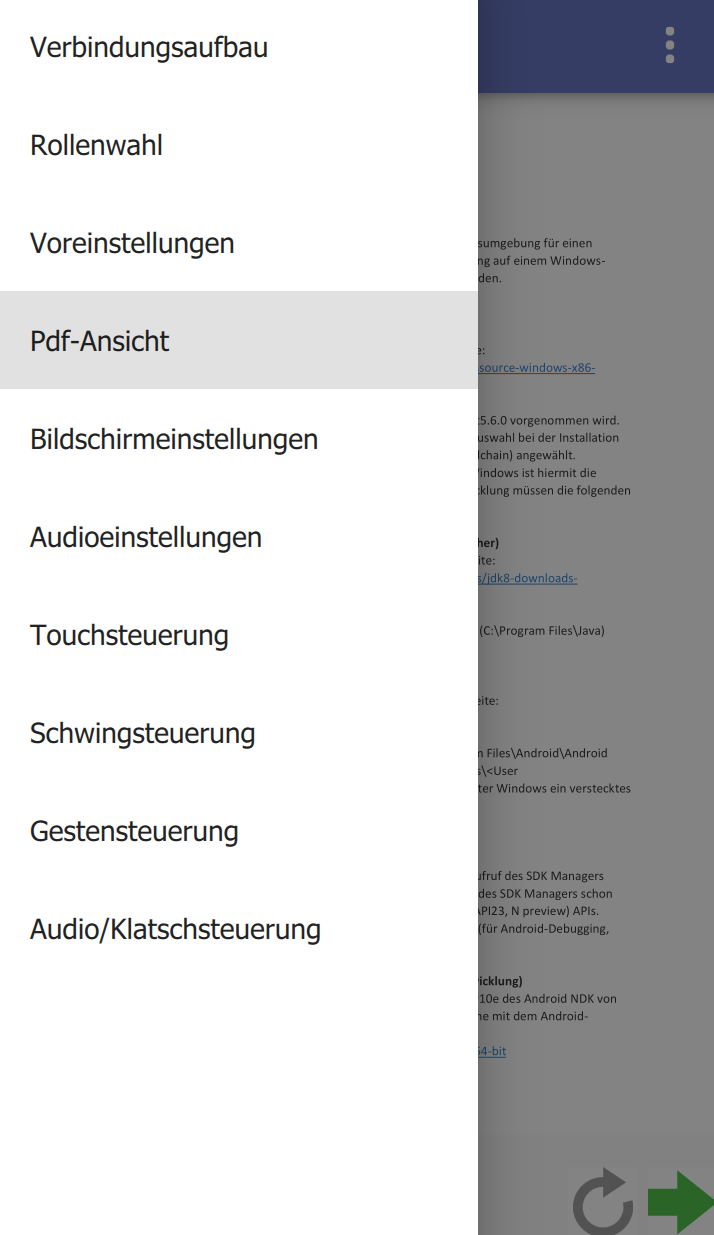
\includegraphics[scale=0.5]{GUI/Bilder/6_Menu-Button_Drawer_mit_Listview.PNG}
	\end{minipage}
	\caption{v.l.n.r.: Voreinstellungen des Zuhörers, PdfAnsicht und Drawer{\tiny}}
	\label{client:H_VoreinstellungenPdfAnsichtDrawer}
\end{figure}

\newpage

\paragraph{Voreinstellungen als Zuhörer}$\;$\\
Als Zuhörer sind die Voreinstellungen ähnlich, jedoch entfällt die Passworteingabe und Herunterladen einer Pdf-Datei ersetzt den Vorgang des Hochladens (siehe \autoref{client:H_VoreinstellungenPdfAnsichtDrawer}). Hierbei erfolgt (ohne eine Auswahlmöglichkeit) das Herunterladen der zuletzt auf dem Server geladenen Datei.
\paragraph{Pdf-Ansicht}$\;$\\
Bestätigen der Voreinstellungen des Sprechers oder Zuhörers bedingt einen Kontextwechsel zur Pdf-Ansicht (siehe \autoref{client:H_VoreinstellungenPdfAnsichtDrawer}).
\paragraph{Drawer}$\;$\\
Ab der Pdf-Ansicht ist der grüne Pfeil oben links durch einen weiteren aus drei waagerechten Strichen bestehenden Menü-Button ersetzt. Dieser Button öffnet eine vertikale Leiste (Drawer) am linken Bildschirmrand, welche ein ListView beinhaltet, dass schnelle Navigation zu allen bisherigen Ansichten und Weiteren ermöglicht (siehe \autoref{client:H_VoreinstellungenPdfAnsichtDrawer}). Durch wischen am vom linken Bildschirmrand nach rechts lässt sich dieser ebenfalls einblenden. Die Navigation über das ListView im Drawer ist nur möglich solange man nicht zu vorherigen Ansichten wechselt. 
\paragraph{Symbolleiste}$\;$\\
Die Pdf-Ansicht beinhaltet ein Symbolleiste (siehe \autoref{client:Symbolleiste}) als Reihe von Icons am unteren Bildschirmrand. Mit ihr ist durch die Pfeile außen ein Blättern in der Pdf möglich. Intuitiv blättert der linke Pfeil zurück, der Rechte vor. Die anderen Buttons dienen dem aktivieren/deaktivieren von Bedienoptionen. Grün signalisiert hierbei aktiviert und grau deaktiviert. Das Mikrofon steht für die Audiosteuerung, das Kamerasymbol für  Gestensteuerung und das Männchen mit den ausgestreckten Armen und Beinen im Kreis für die Kippsteurung. Neben diesem Symbol steht die Seitennummer der angezeigten Seite.
\\Die ineinander greifenden Pfeile signalisieren bei grün, dass die Autosynchronisation aktiv ist. Sobald diese nicht aktiv ist, erscheint ein weiterer Pfeil geschlungen im Uhrzeigersinn in grau auf der Symbolleiste links neben dem Pfeil. Die Funktion ist das manuelle Aktualisieren der Seitenzahl. Ein Sprecher sendet mit dem Refresh-Button die Seitenzahl, die auf seinem Device aktuell ist zum Server, und dieser leitet sie an die Zuhörer-Clients weiter. Ist als Sprecher Autosynchronisation aktiviert, geschieht die bei jedem Blättern automatisch. Zuhörer können über Refresh die aktuelle Seite manuell anfragen oder mit Autosynchronisation alle 2 Sekunden zu der aktuellen Seite zurück springen. Wenn der Sprecher Blättert, erhalten die Zuhörer jedoch in jedem Fall die aktuelle Seite.

\begin{figure}[ht!]
	\centering
	
\includegraphics[scale=0.5]{GUI/Bilder/SchnellLeiste.PNG}
	\caption{Symbolleiste{\tiny}}
	\label{client:Symbolleiste}
\end{figure}

\paragraph{Informationen zur Benutzung}$\;$\\
Da das bisherige Hilfe-Pop-Up nur recht allgemeine Informationen enthält sowie für weitere Hilfestellung auf diese eventuell nicht zur Hand liegenden Dokumentation verweist, kann sich der Benutzer über den Drawer zu einer Erklärung der Bedienmöglichkeiten navigieren. Diese Möglichkeit soll einen möglichst einfachen Einstieg ohne viel ausprobieren sicherstellen und Anwendungsfehler verhindern. Um einen mit dieser Anwendung vertrauten Anwender nicht nach jedem Start durch diese Informationen zu führen, ist das Aufrufen optional (siehe \autoref{client:Symbolleiste}).

\begin{figure}[ht!]
	\centering
	\begin{minipage}{0.31\linewidth}
		\centering
		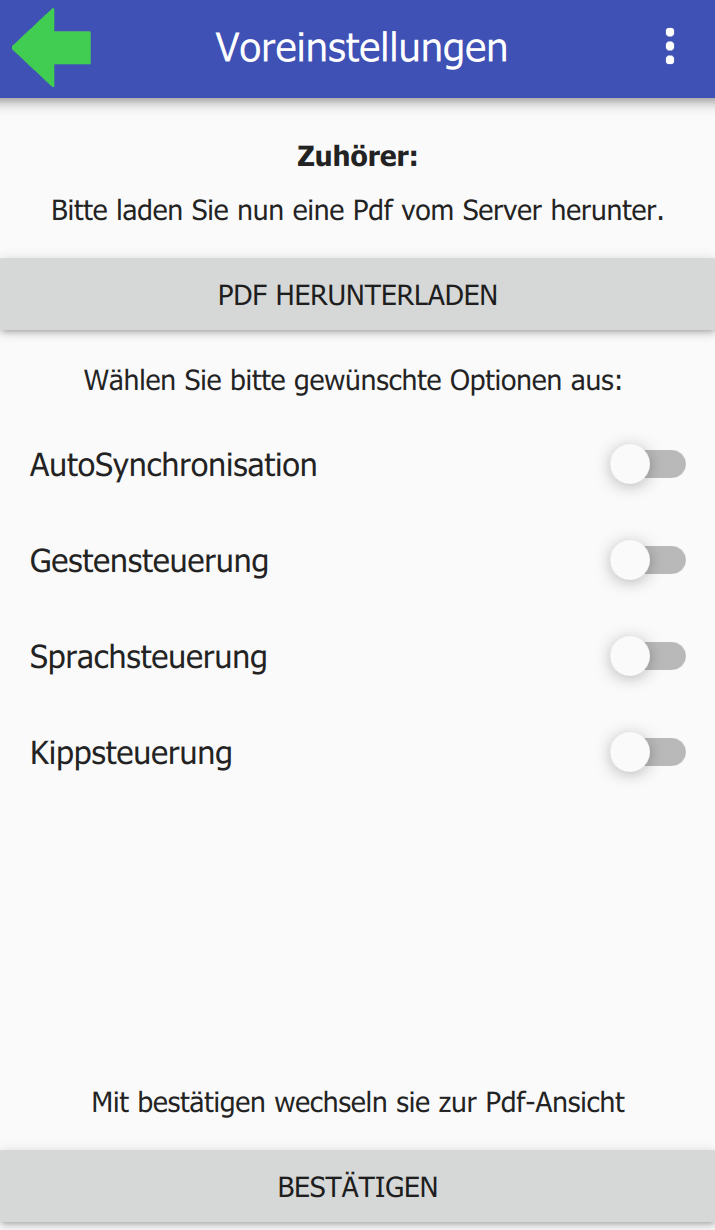
\includegraphics[scale=0.5]{GUI/Bilder/7_H_Voreinstellungen.PNG}
	\end{minipage}
	%\hfill
	\begin{minipage}{0.31\linewidth}
		\centering
		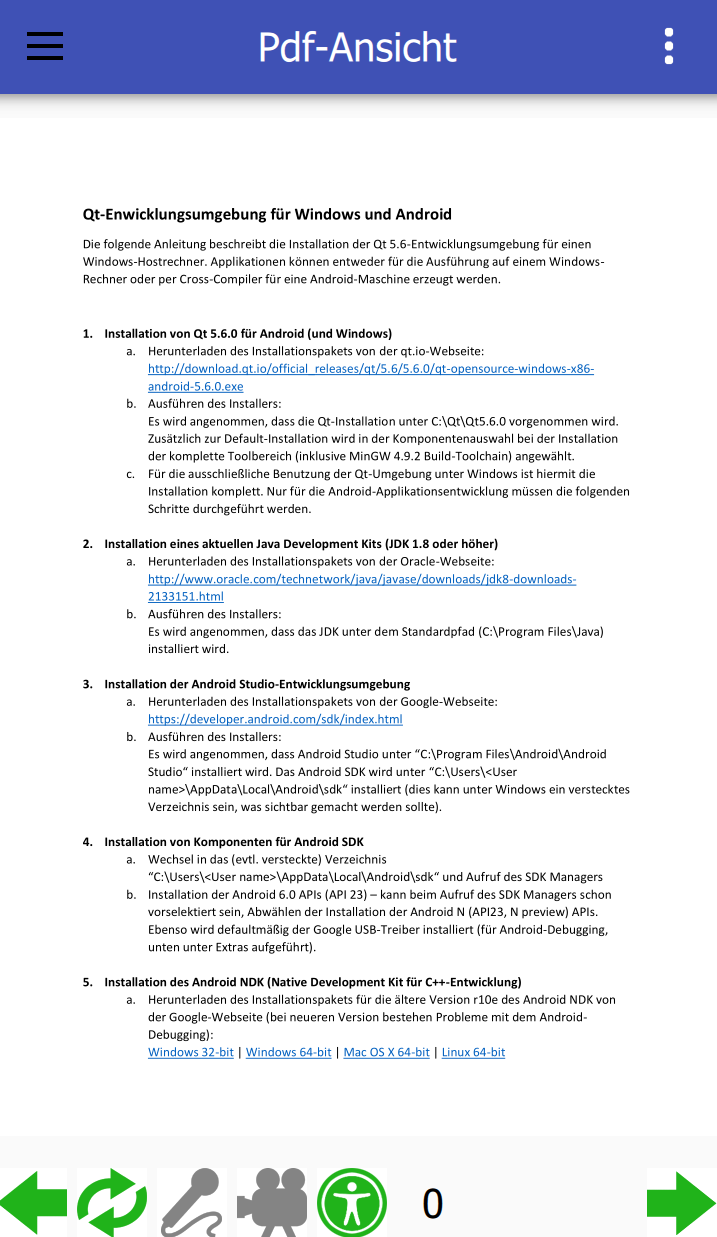
\includegraphics[scale=0.5]{GUI/Bilder/4_S_PDF-Ansicht.PNG}
	\end{minipage}
	\begin{minipage}{0.31\linewidth}
		\centering
		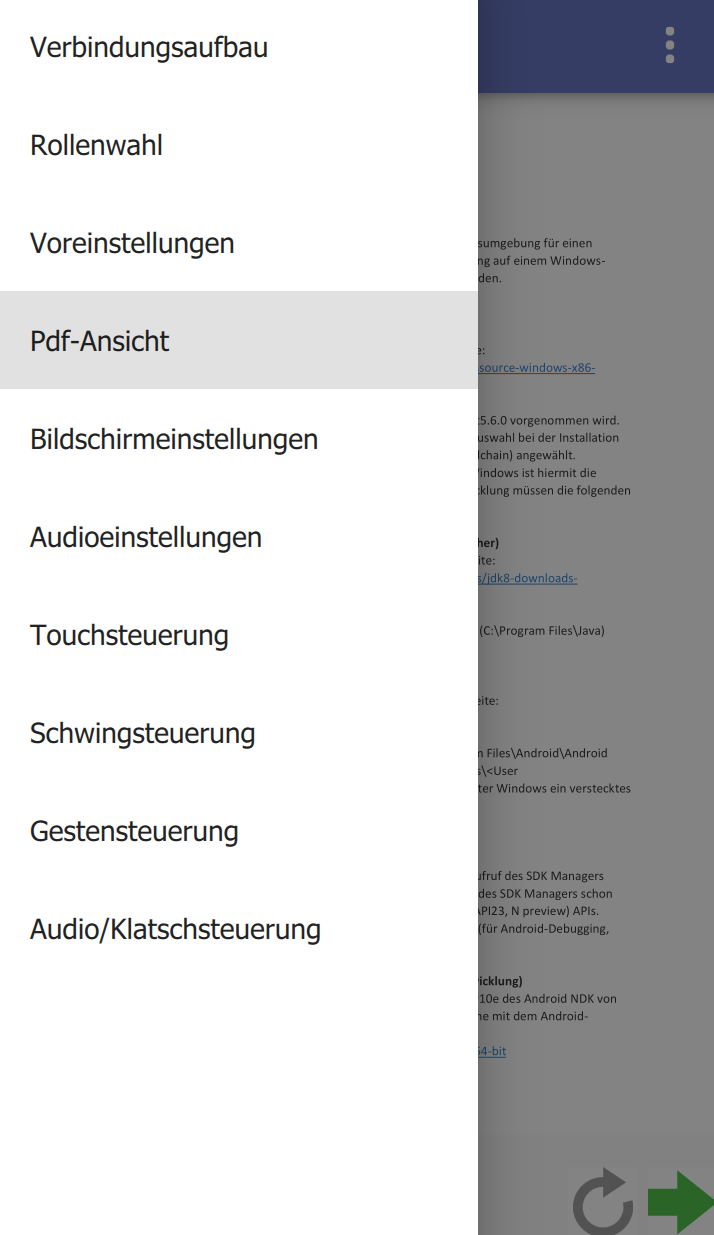
\includegraphics[scale=0.5]{GUI/Bilder/6_Menu-Button_Drawer_mit_Listview.PNG}
	\end{minipage}
	\caption{v.l.n.r.: Gestensteuerung, Kippsteuerung und Klatschsteuerung{\tiny}}
	\label{client:InformationenBedienhilfen}
\end{figure}



\section{Kommunikation}
Die Kommunikation des Clients mit dem Server ist in 
\section{Software}
Die Software finden Sie in Git.

\paragraph{Konzept}$\;$\\
Das Softwarekonzept dient der Umsetzung des Bedienkonzepts mit "Qt-Creator" programmiert in C++ und Qml. Der Qt-Creator ist dafür wegen der Plattformunabhängigkeit ausgewählt.

\paragraph{Struktur}$\;$\\

\paragraph{Zustandssteuerung}$\;$\\
Die Realisierung der Grafische Oberflächen entsprechend bisheriger Einstellungen ist über Zustände einer Variablen "appState" realisiert, die sich die aktuellen Einstellungen bzw. den Ort merkt und entsprechend Informationen mittels der Objekteigenschaft "visible" ein oder ausblendet.
\paragraph{Elemente}$\;$\\
\paragraph{Einbindung der erweiterten Bedienmöglichkeiten}$\;$\\
\paragraph{Details}$\;$\\
\paragraph{Lektionen}$\;$\\

\section{Navigation}

\section{Features}
- Blättern in einer Pdf ohne dass ein Update auf dem Server erfolgt\\
\\INOF ans TEAM:Diese Section ist noch nicht fertig
\section{Erweiterungspotential}
Einige zusätzliche Funktionalitäten könnten, den Wert der Applikation für Zuhörer und Sprecher steigern.\\
\\INOF ans TEAM:Diese Section lade ich später hoch
\\INOF ans TEAM:Wenn Ihr die Zuverlässigkeit der Gestensteuerung, Kippsteuerung, Audiosteuerung oder die Sicherheit der Kommunikation noch verbessern wollt, könnt ihr ja wie Tim es in euren Abschnitt einfügen. Hier geht es nur um Erweiterungen der allgemeinen mögliche Funktionalität der Clientapp wie Puplikumsfragen oder sowas.
Erweiterungen für den Sprecher:\\

Erweiterungen für den Zuhörer:\\
- Einstellen der Zeit die vergehen soll bis sich die Applikation synchronisiert\\






\newpage
So kann Code eingefügt werden.
\begin{lstlisting}[frame=single,breaklines=true,basicstyle=\tiny,language=C,label={PWMStart},caption={Kommentierter Start der PWM}]
/*! \brief Starts the PWM
* 
* To make sure that the PWM behaves correctly after a Compare Bit Change the PWM is started and reset with a software trigger.
*/
static void vStartPwm( void )
{
tc_start( &AVR32_TC0, PWM_CHANNEL );
tc_software_trigger( &AVR32_TC0, PWM_CHANNEL );
}
\end{lstlisting}